%%%%%%%%%%%%%%%%%%%%%%%%%%%%%%%%%%%%%%%%%
% Journal Article
% LaTeX Template
% Version 1.0 (25/8/12)
%
% This template has been downloaded from:
% http://www.LaTeXTemplates.com
%
% Original author:
% Frits Wenneker (http://www.howtotex.com)
%
% License:
% CC BY-NC-SA 3.0 (http://creativecommons.org/licenses/by-nc-sa/3.0/)
%
%%%%%%%%%%%%%%%%%%%%%%%%%%%%%%%%%%%%%%%%%

%----------------------------------------------------------------------------------------
%	PACKAGES AND OTHER DOCUMENT CONFIGURATIONS
%----------------------------------------------------------------------------------------

\documentclass[twoside]{article}
\usepackage{etex}
\usepackage{pgfplots}
\usepackage{cite} % Better citations
\usepackage{setspace}
\usepackage{mathtools}
\usepackage[sc]{mathpazo} % Use the Palatino font
\usepackage[T1]{fontenc} % Use 8-bit encoding that has 256 glyphs
\linespread{1.00} % Line spacing - Palatino needs more space between lines
\usepackage{microtype} % Slightly tweak font spacing for aesthetics
\usepackage{graphicx}
%\usepackage[hmarginratio=1:1,top=16mm,columnsep=20pt]{geometry} % Document margins
\newcommand{\bigO}{\ensuremath{\mathcal{O}}}
\usepackage[headsep=0.05in,scale=1.0,margin={0.5in,0.5in},columnsep=20pt]{geometry}
%\oddsidemargin 0.0in %%this makes the odd side margin go to the default of 1inch
%\evensidemargin 0.0in
%\headheight 0.5in
%\topmargin 0.5in
%\textheight 9.0in
%\textwidth 6.5in %%sets the textwidth to 6.5, which leaves 1 for the remaining right margin with 8 1/2X11inch paper 

\usepackage{multicol} % Used for the two-column layout of the document
%\usepackage{hyperref} % For hyperlinks in the PDF

\usepackage[hang, small,labelfont=bf,up,textfont=it,up]{caption} % Custom captions under/above floats in tables or figures
\usepackage{booktabs} % Horizontal rules in tables
\usepackage{float} % Required for tables and figures in the multi-column environment - they need to be placed in specific locations with the [H] (e.g. \begin{table}[H])
\usepackage{lettrine} % The lettrine is the first enlarged letter at the beginning of the text
\renewcommand{\LettrineTextFont}{\rmfamily}
\usepackage{paralist} % Used for the compactitem environment which makes bullet points with less space between them

\usepackage{abstract} % Allows abstract customization
\renewcommand{\abstractnamefont}{\normalfont\bfseries} % Set the "Abstract" text to bold
\renewcommand{\abstracttextfont}{\normalfont\small\itshape} % Set the abstract itself to small italic text

\pagestyle{plain} % no page numbers in footer
\usepackage{scalefnt} %scale font for title
\usepackage{titlesec} % Allows customization of titles
\usepackage{comment}	%Allows addition of comments
%\usepackage[small,compact]{titlesec}
\titleformat{\section}[block]{\large\scshape\centering{\Roman{section}.}}{}{1em}{} % Change the look of the section titles 

%----------------------------------------------------------------------------------------
%	TITLE SECTION
%----------------------------------------------------------------------------------------

%\title{\vspace{-15mm}\fontsize{20pt}{5pt}\selectfont\textbf{Experienced Search}} % Article title

%----------------------------------------------------------------------------------------

\begin{document}
%\title{\vspace{-20mm}{On-Line Recognition of Continuous Mouse Gesture Sequences}}
%\date{}
%\maketitle % Insert title
\scalefont{2}
\centerline{Recognition of Unistroke Gesture Sequences}
\normalsize

%----------------------------------------------------------------------------------------
%	ARTICLE CONTENTS
%----------------------------------------------------------------------------------------

\begin{multicols}{2} % Two-column layout throughout the main article text

\section{Problem Statement}
\lettrine[nindent=0em,lines=2]{G}estures are a popular and growing form of input
in human-centric user interfaces, primarily due to their natural use in everyday
communication \cite{mitra_gesture_2007}.
One important domain where gestures are frequently encountered is law
enforcement, where a significant concern is recognition of gang symbols in
graffiti and other forms of hand-written communication. The United States
Federal Bureau of Investigation's Safe Streets and Gang Unit commonly encounters
handwritten communication using custom
gestures\cite{lyddane_donald_united_2006}. The key features of law enforcement's
gesture identification problem are 1) recognition of previously-identified
custom symbols, and 2) identification of those symbols within a gesture
sequence.

Recognizing a sequence of symbols is difficult primarily because of the
segmentation problem, that is, the problem of analyzing a gesture sequence and
identifying where each individual gesture begins and ends.
It is useful to compare the problem we are interested in tackling with similar
problems. Unlike the problem of letter identification in written languages, the sequence
of gestures doesn't follow a well-defined grammar. However, similar to the
problem of letter recognition in cursive handwriting, our gesture sequences have
no obvious ``breaks'' to demarcate individual gestures. In the next section, we
review work related to this problem.

%Problem addressed and its importance
%    ⁃    poor: does not mention problem or does not say why it is important
%    ⁃    acceptable: problem is tied to societal needs and backed up with reasons
%    ⁃    exceptional: succeeds in really convincing the reader (way beyond lip service)

%------------------------------------------------
\section{Related Work}

The related work focuses on problems similar to ours, but with some key
differences. In this section, we review related problems, and the
approaches taken, in order to compare and contrast each approach with ours.

Yang et al \cite{yang_gesture_1994} present work on recognition of individual
gestures in continuous gesture sequences containing arbitrary gestures (e.g.,
digits). The notable difference between their work and ours is the problem
approach. They train HMMs to recognize continuous gesture sequences defined
\textit{a priori}, and, because of their use of HMMs, require an intensive
training period, both of which we see as deficiencies.

Hong et al, in their paper on Chinese character recognition
\cite{hong1998segmentation}, use a two-level iterative segmentation technique
that uses whitespace separation to split character sequences into individual
characters. Their approach does not work for our problem, where gestures are drawn in one
continuous motion, uninterrupted by white space.

Robust individual gesture recognition systems exist, such as the mouse gesture
recognition system developed by Tanguay\cite{tanguay_jr_hidden_1995}. However,
the implementation is tailored to individual gesture recognition, and does not
extended easily to recognize unistroke gesture sequences.

The \$1 recognizer \cite{wobbrock2007gestures} is a single gesture recognition
system which works even without any training by the user (the system has a
built-in gesture set which can be supplemented with additional training data
tailored for the individual user). The primary deficiency of this system is its
inability to recognize sequences of gestures.

%------------------------------------------------
\section{Approach}

%Approach (What was done?)
%    ◦    poor: minimal description, hard to understand/replicate
%    ◦    acceptable: is specific about what was implemented and explains it well
%    ◦    exceptional: well written, clear explanations, reproducible: you care about the reader!

In order to study the problem of segmentation of a gesture sequence, we created
a web-based prototype of a gesture recognition environment using mouse-based
input, inspired by (and derived from) the \$1 recognizer web-based
application\cite{wobbrock2007gestures}.

During system use, the user chooses gestures from the pre-defined gesture list, trains the selected gestures by drawing
the individual gestures, and then draws 1, 2, or 3 arbitrary gestures as
a single unistroke gesture sequence.

There are two states in our prototype gesture recognizer: (1) a training state,
where the user selects a gesture, and trains the chosen gesture by replicating
it and adding the data as a gesture template, and (2) a recognition state, where
the user draws a unistroke gesture sequence for subsequent recognition.

A screenshot of the system in the recognition state is shown in the following figure:

\begin{figure}[H]
	\centering
	\includegraphics[height=6cm, width=9cm]{Images/GUI.png}
	\label{fig1}
	\caption{Recognition GUI}
\end{figure}
  
Our approach, at a high level, is very straightforward, and divided into two
main steps. The first step is to match each individual gesture against a portion
of the input data, thereby segmenting the unistroke gesture sequence into the
first gesture, and the remaining input. The second step is to remove the first
gesture from the input sequence and iterate, searching for additional gestures.
The difficult part is accurately segmenting the unistroke sequence. The following
section details our segmentation approach.

\subsection*{Segmentation}

The main challenge in our
approach was to come up with a technique which was neither too strict (as users
generally are unable to repeatedly reproduce gestures exactly) nor too lenient
(we do not want to recognize noise as a gesture). Additionally, we need an approach
that is fairly robust to segmentation ambiguities. Because users are not constrained in their choice of gestures,
ambiguity can exist regarding the appropriate segmentation of a gesture sequence, as shown
in Figure 2: 

\begin{figure}[H]
	\centering
	\includegraphics[height=5cm, width=5.5cm]{Images/Ambiguity1.png}
	\label{fig2}
	\caption{Ambiguity in gesture recognition}
\end{figure}

During recognition, the user draws a unistroke gesture sequence, which is recorded as an ordered
list of $(x,y)$ coordinates. It is this sequence of ordered points that is
inspected for potential matches of individual gestures. First, each
gesture recorded in the system is logically identified, and each sample of that
logical gesture (a ``template") is compared with the user's input, as follows.
The template gesture is resampled to $64$ equidistant points in order to provide
a basis for direct pointwise comparison with the user input. Resampling is
essential when comparing templates of \emph{individual} gestures against the
user input, which may contain \emph{one or more} individual gestures. A
fundamental insight into the problem that justifies our approach is that a
sequence of gestures is going to ``contain more data'' (i.e., have a longer 2-D
path length) than a single gesture. In addition to resampling the template
gesture, the user's input is also resampled, primarily to smooth out natural
variations (jagged edges, etc.) in user input. We found that $64$ points was
both high enough to retain the resolution necessary to disambiguate gestures and
low enough to be computationally inexpensive. Additionally, this number has
been used and suggested in the \$1 Recognizer\cite{wobbrock2007gestures}.

After resampling, the path length of the template is calculated and a threshold
is set at $90\%$ of the full path length. The purpose of the threshold is to
ensure that we don't require the full template data set to appear in the user's
input, which we felt was an intuitive and valid consideration (to see this,
simply consider the scenario for a gesture sequence of length $1$). The next
step is to calculate the corresponding number of points in the user's input
whose path length approximately equals the thresholded template path length.
Note that if $90\%$ of the full path length is longer than the path length of
the user input, the candidate gesture is deemed to not be a potential match, and
skipped.

We now have a portion of the user input that may match a gesture template. To
determine a quantitative measure, we first translate both the user's input and
the template to the origin and compare the segments pointwise using dynamic time
warping (briefly reviewed in the next section).
At this point, we have a candidate segment of user input with a score, but not
necessarily a minimal score. To determine a minimal score, we search both
backward and forward in the user input for a better match (indicated by a lower
score). As long as the score of the tested segment is better than the previous
score, we continue searching backward (forward) in the user input. The minimal
score is computed, and retained for comparison against all other templates.

All of the candidate templates for the possible individual gestures are
identified in this manner and then sorted in order of ascending score. The
minimal score is the best match, and this is the gesture chosen as the first in
the user's input. An example of the results of this segmentation process is
shown above in Figure 1.

\subsection*{Dynamic Time Warping}

As mentioned above, our algorithm for matching individual gestures is dynamic time warping (DTW).
DTW is appropriate due to our need for flexible matching of resampled input and template
gestures. DTW essentially minimizes a distance calculation between two inputs X and Y,
where each input is sampled over time. DTW ``warps" time to map each sample in X and Y to
the ``closest" match (as measured by the DTW distance calculation). Recall that our inputs
have differing numbers of sample points (the template is resampled to $64$ points, but a
segment of the user's input, less than or equal to the resampled $64$ points, is chosen
to compare with the template). For our 2-D data, the appropriate distance metric is Euclidean distance:

\[
 dist = \displaystyle\sqrt{(x_1-x_2)^2 + (y_1-y_2)^2}
\]

Using the minimal cost of neighboring points (we compare three nearby dtw calculations),
we map each point \emph{i} in input X to a nearest point \emph{j} in input Y.

%------------------------------------------------
\section{Evaluation}

%Evaluation (What were the results)
%    ◦    poor: just a qualitative assessment, no real results/numbers given
%    ◦    acceptable: qualitative as well as quantitative results, organized in tables and/or figures
%    ◦    exceptional: above and beyond in making the reader understand (not yet interpret) the results

The unique component of our system is our segmentation routine, but is is tightly coupled (and dependent upon) the accuracy of the individual gesture recognition (DTW). As a result, we evaluated our recognition system via three metrics:
\begin{enumerate}
\item Overall Accuracy: This is an all-or-nothing measure. For input sequence of
lengths 1, 2 or 3, we measured the percentage of trials in which the system
output both the correct number and correct identity of individual gestures.

\item
Segmentation Accuracy: For input sequence of lengths 1, 2 or 3, we measured the
percentage of trials in which the system output the correct \emph{number} of
gestures (regardless of correct identification of individual gestures).

\item Relaxed Accuracy: This is a relaxed version of Overall Accuracy relevant
only to input containing multiple gestures. For input sequences of length 2 or 3,
we measured the number of gestures in the output that actually appear in the input, accounting for order.
The purpose of this metric is to measure output where the incorrect number of gestures was identified, or perhaps where the segmentation routine did not ``correctly segment" each gesture, but where the segmentation correctly segmented part of the input gesture sequence.
For this metric, we count the first gesture in the input that is correctly identified, count that gesture as $+1$ and continue
summing over the rest of the output. For example, if the input unistroke gesture sequence is $check, star, \{$, and the system
outputs the sequence as $v, star, \{$, the
Relaxed Accuracy = 2, counting both the $star$ and the $\{$. If the same sequence was identified as $check, v, [$, the Relaxed
Accuracy = 1 (counting the $check$). Finally, if the sequence was identified as $v, star, caret, \{$, the Relaxed Accuracy = 2 (counting the $star$ and $\{$).
The score assigned to a particular trial is:
\[
		Relaxed Accuracy = \frac{\text{Reported gestures in the input}}{\text{Total gestures in the input sequence}}
	\]
\end{enumerate}

We conducted a micro-study involving three third-party users who conducted
multiple recognition phases. Each study participant first chose 5 gestures out
of the set of 16 to use for the study. Then the participant entered a
recognition phase, where they drew 10 unistroke gesture sequences of lengths 1,
2, and 3 (using the 5 chosen gestures). After the first recognition phase, the participant trained each of the
5 chosen gestures once, and then re-entered the recognition phase. The user
alternated training and recognition phases two more times, training each of the
5 gestures a total of 3 times (during the second training phase) and then 5 times (during the third training phase).

We calculated the three accuracy metrics for the aggregate data. The results are shown in Tables 1,2 and 3 respectively.

\begin{table}[H]
  \centering
  \caption{Overall Accuracy}
    \begin{tabular}{rr}
    \toprule
    Sequence Length & Accuracy Rate \\
    \midrule
    1     & 90\% \\
    2     & 50\% \\
    3     & 20\% \\
    \bottomrule
    \end{tabular}%
  \label{tab:addlabel}%
\end{table}%

\begin{table}[H]
  \centering
  \caption{Segmentation Accuracy}
    \begin{tabular}{rr}
    \toprule
	Sequence Length & Segmentation Accuracy \\
    \midrule
    1     & 100\% \\
    2     & 80\% \\
    3     & 60\% \\
    \bottomrule
    \end{tabular}%
  \label{tab:addlabel}%
\end{table}%

\begin{table}[H]
  \centering
  \caption{Relaxed Accuracy}
    \begin{tabular}{rr}
    \toprule
    Sequence Length & Accuracy Rate \\
    \midrule
    2     & 50\% \\
    3     & 50\% \\
    \bottomrule
    \end{tabular}%
  \label{tab:addlabel}%
\end{table}%

Lastly, we gained insight into the effect of training additional templates for each of the chosen gestures by measuring the Overall Accuracy (for sequences of length 1) and Relaxed Accuracy (for sequences of lengths 2 and 3) for the different phases of the study. The results are shown in Figure 3.

\begin{figure}[H]
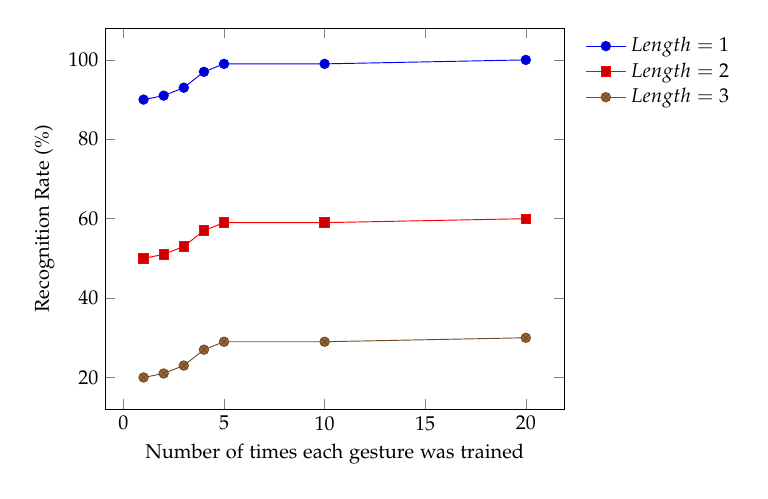
\begin{tikzpicture}[thick,scale=0.85, every node/.style={scale=0.85}]
    \begin{axis}[
	    legend pos= outer north east,
	    legend style={draw=none},
        xlabel=Number of times each gesture was trained,
        ylabel=Recognition Rate (\%)
    ]
      \addplot plot coordinates {
        (1,     90)
        (2,    91)
        (3,    93)
        (4,   97)
        (5,   99)
        (10,   99)
        (20,  100)
    };

      \addplot plot coordinates {
        (1,     50)
        (2,    51)
        (3,    53)
        (4,   57)
        (5,   59)
        (10,   59)
        (20,  60)
    };

      \addplot plot coordinates {
        (1,     20)
        (2,    21)
        (3,    23)
        (4,   27)
        (5,   29)
        (10,   29)
        (20,  30)
    };
    
    \legend{$Length=1$\\$Length=2$\\$Length=3$\\}
    \end{axis}
\end{tikzpicture}	
	\caption{Recognition Rate Vs. Size of Training Data}
	\label{fig3}
\end{figure}

%------------------------------------------------
\section{Discussion}

% Discussion (How to interpret the results)
%    ◦    poor: discusses and interprets the numbers and figures in the Evaluation Section
%    ◦    acceptable: in addition speculates about deeper reasons and/or insight into the algorithms that provides a better understanding to the reader
%    ◦    exceptional: additionally reflects on the entire project, discussing what you have learned, what you would change about what you did, and what possible additional work on this topic might be interesting

Glancing at Tables 1, 2 and 3 together, it is apparent that our segmentation
method yields reasonable, but far from perfect, results. The accuracy rate for
sequence length 1 of ``JDP TODO" as shown in Table 1 confirms that DTW is an
excellent choice of algorithm for matching two data sets that vary in time,
which is exactly the variance we encounter when recognizing individual gestures.
This fact becomes clearer when we compare the DTW approach to the HMM approach taken by Tanguay \cite{tanguay_jr_hidden_1995}, where he
achieved a recognition accuracy of
$60-70\%$ on lower-case English alphabet letters after extensive training.

Table 1 shows a drop-off in accuracy as the sequence length increases. This
drop-off indicates a fundamental shortcoming in our approach: improper
recognition of a gesture results in an improper segmentation, and thus Overall
Accuracy clearly reflects the ``all or nothing" nature of our approach. A
comparison for our results of sequences of length 2 is with the results presented by Yang et
al \cite{yang_gesture_1994}. They report a nearly perfect recognition rate of up to 99.78\%.
The differences in the approaches (motivated by the differences problem statements, as detailed above), are a key consideration when comparing these numbers.
Yang et al train Hidden Markov models for both individual gestures as well as
for all possible 2-gesture combinations. The comparison clearly shows that reducing our problem ``complexity'' by training on gesture sequences should yield significantly improved recognition rates.

Table 2 indicates that our algorithm was able to recognize the correct number of
gestures in input sequences of length 1 80\% of the time.
This implies that our segmentation routine itself is interfering with simply
matching each template against the entire input sequence, and comparing that
score against the ``predicted segmentation''.
Additionally, comparing the segmentation percentages for lengths 2 and 3 found
in Table 2 with the corresponding Overall Accuracy rates in Table 1 reveals that
our segmentation algorithm is identifying the correct number of gestures in
cases where it doesn't correctly identify each individual gesture exactly.

Note that the data in table 2 is closely related to the data in table 1. In
particular, table 2 shows the percentage of trials (broken down by length) that
were correctly segmented into the approprate number of gestures. The data in
Table 1 shows the percentage of trials that were completely recognized. Note
that the trials counted in Table 1 are a proper subset of the trials counted in
Table 2. As a result, one can conclude that the difference in Overall Accuracy
as compared to Segmentation Accuracy is due to incorrect recognition of
individual gestures. Thus, this implies that a more robust technique for
individual gesture recognition would significantly boost the Overall Accuracy.

The Relaxed Accuracy results in Table 3 indicate that the system is
``recovering" after it incorrectly identifies a gesture in the sequence.
Specifically, when comparing the results for gestures of length 2 in Table 3 to
the corresponding results in Table 1, the higher Relaxed Accuracy rate indicates
that the system is more often able to correctly recognize one gesture in the
sequence.
This is noteworthy primarily because it implies that training to
``dis-ambiguate'' gestures (in particular, gestures that the user did not use
but that were available in the system) may prove effective. The results for
length 3 are similar.

Figure 3 clearly shows that additional training benefits Overall Accuracy (for
length 1) and Relaxed Accuracy (for lengths 2 and 3) considerably.
This result matches the intuition of the effect of tightly coupling the
segmentation routine and the DTW algorithm. Increasing recognition rates
increases the ability for the segmentation routine to properly match each
gesture, and thus properly segment the gesture sequence.

%shows that we do not require a lot of training data to get a good
%recognition rate. Even if each gesture has just one template instance during the
%training phase, we were able to achieve 90\%, 50\% and 20\% recognition accuracy
%for 1-gesture, 2-gesture and 3-gesture input sequences. Also we observe that by
%increasing the number of training samples, we were able to improve on the
%accuracy, but this improvement was incremental most of the time. It goes to show
%that the role of the training phase in our approach is minimal.


% JDP BEGIN

The primary lessons we learned from our project are as follows. First, we
observed during the study that the gestures themselves were drawn differently
during training (when gestures were drawn individually) and during
recognition (when gestures were drawn as part of a gesture sequence). This
observation is consistent with other research results that indicate
that a complex motion is ``more than the sum of its parts", or more formally,
that the transition between gestures in a gesture sequence is critical
data that can be used to dis-ambiguate potential gesture segmentation choices.
The second important lesson is that training on gesture sequences is very likely
to yield impressive accuracy gains. This lesson is indicated primarily by
comparing with related work (Yang et al).

Regarding future work, our preferred approach to achieving the highest accuracy
rates for our current problem definition would be to use HMMs and train on
gesture sequences. Additionally, it would be worthwhile to ease the problem
constraints and allow the user to intentionally provide ``segmentation cues"
during a unistroke gesture sequence. A simple, relatively non-intrusive cue
would be a deliberate pause between gestures in a sequence (which, as an aside,
occurred naturally during the study).

%----------------------------------------------------------------------------------------
\section{References}

\begin{spacing}{0.9}
%\scalefont{0.9}
\bibliographystyle{unsrt}	
%\bibliography{myrefs}
\begingroup
\renewcommand{\section}[2]{}%
\bibliography{myrefs}
\endgroup
\end{spacing}
%\normalsize

\end{multicols}
\end{document}

%	Member #1: Justin Permar - GT ID:902931271
%	Member #2: Arvind Krishnaa Jagannathan - GT ID: 902891874
%